\documentclass{beamer} % blue; brown; gray; red;
\usepackage{beamerthemesplit}
\usepackage{beamerthemeshadow}
\usepackage{animate}
\usepackage{hyperref}
\usepackage[inline]{asymptote}
%\usepackage[numbered]{mcode}
\usepackage{graphics}
\usepackage{colortbl}
\usepackage{pgf,pgfarrows,pgfnodes,pgfautomata,pgfheaps}
\usepackage{amsmath,amssymb}
\usepackage{overpic}
\usepackage{calc}
\usepackage{ifthen}
\usepackage{tikz,pgfplots}
\usetikzlibrary{shapes,arrows}
\usetikzlibrary{shapes.multipart}
\usetikzlibrary{positioning}
\usetikzlibrary{automata,calc}
\usepackage{verbatim}
\usepackage{algorithm}
\usepackage{algorithmic}
\usepackage{fixltx2e}
\pgfdeclarelayer{background}
\pgfsetlayers{background,main}
\usetikzlibrary[arrows,decorations.pathmorphing,backgrounds,positioning,fit,petri]

%%%%%%%%%%%%%%%%%%%%%%%%%%%%%%%%%%%%%%%%%%%%%%%%%%%%%%
\usepackage{xeCJK}
%\usepackage{fontspec}
\setCJKmainfont[BoldFont=simhei.ttf]{simkai.ttf}
%\setCJKsansfont{simhei.ttf}
%\setCJKmonofont{simfang.ttf}
%%%%%%%%%%%%%%%%%%%%%%%%%%%%%%%%%%%%%%%%%%%%%%%%%%%%%%

\usetheme{Warsaw}
%别的主题:Bergen,Boadilla,Madrid,AnnArbor,CambridgeUS,Pittsburgh, Rochester.
%有导航栏:Antibes,JuanLesPins,Montpellier,
%有内容的:Berkeley,PaloAlto,% Goettingen,Marburg,Hannover
%小导航栏:Berlin,Ilmenau,Dresden,Darmstadt, Frankfurt,Singapore,Szeged,
%章节表单:Copenhagen,Luebeck,Malmoe,Warsaw
\beamertemplateshadingbackground{red!10}{structure!10}
\beamertemplatesolidbackgroundcolor{white!90!blue}
\beamertemplatetransparentcovereddynamic
\beamertemplateballitem
\beamertemplatenumberedballsectiontoc
%\beamertemplatelargetitlepage
\beamertemplateboldpartpage

\usecolortheme{sidebartab}
%beetle,crane,dove,fly,seagull,wolverine,beaver
\renewcommand{\raggedright}{\leftskip=0pt \rightskip=0pt plus 0cm}
\raggedright
%%%%%%%%%%%%%%%%%%%%%%%%%%%%%%%%%%%%%%%%%%%%%%%%%%%%%%%%%%%%%%%%%%%%%%%%%%
\graphicspath{{figures/}}

\setbeamertemplate{caption}[numbered]
\newcommand{\animatepath}{./animate}
\newcommand\includepart[1]{\include{./part/#1}}
%%%%%%%%%%%%%%%%%%%%%%%%%%%%%%%%%%%%%%%%%%%%%%%%%%%%%%%%%%%%%%%%%%%%%%%%%%
\definecolor{MyDarkGreen}{rgb}{0.0,0.4,0.0}

\renewcommand\contentsname{\bf 目录}
\renewcommand\figurename{\bf 图}
\renewcommand\tablename{\bf 表}
\renewcommand\refname{参考文献}

%%%%%%%%%%%%%%%%%%%%%%%%%%%%%%%%%%%%%%%%%%%%%%%%%%%%%%%%%%%%%%%%%%%%%%%%%%
%% 定义一些自选的模板,包括背景、图标、导航条和页脚等,修改要慎重
\makeatletter
\usefoottemplate{ %重新定义页脚,加入作者,单位,单位图标,和文档标题
  \vbox{\tiny%
    \hbox{%
      \setbox\beamer@linebox=\hbox to\paperwidth{%
        \hbox to.5\paperwidth{
            \hfill\tiny\color{white}
                  \textbf{\insertshortauthor\quad\insertshortinstitute}
            \hskip .1cm\lower 0.2em\hbox{
\includegraphics[height=0.25cm]{./figures/CAS-blue.pdf}}
            \hskip.3cm}%
        \hbox to.5\paperwidth{
            \hskip.3cm\tiny\color{white}
                  \textbf{\insertshorttitle}\hfill}\hfill}%
      \ht\beamer@linebox=2.625ex%
      \dp\beamer@linebox=0pt%
      \setbox\beamer@linebox=\vbox{\box\beamer@linebox\vskip1.125ex}%
      \color{structure}\hskip-\Gm@lmargin\vrule width.5\paperwidth
      height\ht\beamer@linebox\color{structure!70}\vrule width.5\paperwidth
      height\ht\beamer@linebox\hskip-\paperwidth%
      \hbox{\box\beamer@linebox\hfill}\hfill\hskip-\Gm@rmargin}
  }
}
\makeatother
%%%%%%%%%%%%%%%%%%%%%%%%%%%%%%%%%%%%%%%%%%%%%%%%%%%%%%%%%%%%%%%%%%%%%%%%%%
\title{基于耗散粒子动力学的细胞模型和模拟}
\subtitle{工作介绍和展示}
\institute[流固耦合系统力学重点实验室]{流固耦合系统力学重点实验室}
\author{\href{mailto:zhou.lv.wen@gmail.com}{周吕文} (导师:刘谋斌)}
\date{2014年09月26日}
%%%%%%%%%%%%%%%%%%%%%%%%%%%%%%%%%%%%%%%%%%%%%%%%%%%%%%%%%%%%%%%%%%%%%%%%%%
\hypersetup{pdfauthor={周吕文},
            pdftitle={基于耗散粒子动力学的细胞模型和模拟},
            pdfsubject={工作介绍和展示},
            pdfkeywords={耗散粒子动力学,细胞模型},
            pdfproducer={XeLateX with hyperref},
            pdfcreator={Xelatex}}
\begin{document}
\frame[plain]{
\titlepage
} 
\titlegraphic{\pgfuseimage{title}}
\AtBeginSection[]{ % 在每个Section前都会加入的Frame


  \frame<handout:0>{
    \frametitle{提纲}
    \tableofcontents[current,currentsubsection]
  }
}
\frame[Outline,plain]{\frametitle{提纲}\tableofcontents
}
%%%%%%%%%%%%%%%%%%%%%%%%%%%%%%%%%%%%%%%%%%%%%%%%%%%%%%%%%%%%%%%%%%%%%%%%%%

\section{研究方法}
\subsection{耗散粒子动力学简介}
\frame{ \frametitle{耗散粒子动力学简介}
\note{\textcolor{red}{[100-130s]}下面简要介绍一下耗散粒子动力学:}
  \begin{itemize}
  \item 耗散粒子动力学(DPD)是一种粗粒化的分子动力学方法,适合模拟介观尺度的简单和复杂流体动力学和流变性能.
        \note[item]{耗散粒子动力学(DPD)是一种粗粒化的分子动力学方法}
  \item 由Hoogerbrugge与Koelman首先提出, 旨在解决经典分子动力学难以解决的流体
        时间和空间尺度问题.
        \note[item]{提出这一方法的目的是为了解决经典分子动力学难以解决的流体时间和空间尺度问题}
  \item 优点: 与经典分子动力学方法相比, DPD方法可以使用更大的粒子尺寸和更长的时间步长, 因此具有更好的计算效率与计算能力,能应用到介观尺度乃至亚宏观的问题.
        \note[item]{因此相对于经典分子动力学, DPD由于可以使用更大的粒子尺寸和更长的时间步长,而且有更好的计算效率与计算能力.}
  \item 应用: 各类复杂的流体流动, 如相分离, 蛋白质等大分子悬浮, 表面活性剂, 胶
        体输运, 稀释聚合物溶液, 生物薄膜, 以及介观尺度的多相流动现象.
        \note[item]{现在的应用也相当广泛.}
  \end{itemize}
}

\subsection{运动方程}
\frame{\frametitle{运动方程}
\begin{columns}
\begin{column}[c]{0.35\textwidth}
\begin{center}
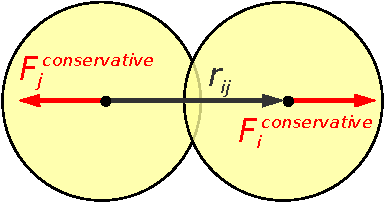
\includegraphics[width=0.9\textwidth]{conservative.pdf}
\vspace{1em}

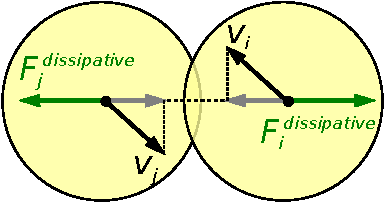
\includegraphics[width=0.9\textwidth]{dissipative.pdf}
\vspace{1em}

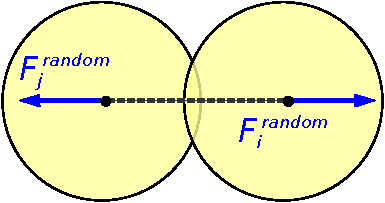
\includegraphics[width=0.9\textwidth]{random.pdf}
\end{center}
\end{column}
\begin{column}[c]{0.65\textwidth}
\note{\textcolor{red}{[130-145s]}}
牛顿运动方程描述DPD粒子运动\note[item]{DPD模型中粒子的运动由牛顿运动方程描述.}
  \[
  \frac{d\mathbf{r}_i}{dt} = \mathbf{v}_i,   
  \frac{d\mathbf{v}_i}{dt} = \mathbf{f}_i = \mathbf{f}_i^{\text{int}} + \mathbf{f}_i^{\text{ext}}
  \]
\note[item]{耗散粒子动力学中的粒子除了受到保守力外, 还受到耗散力和随机力.}
%\note[item]{耗散力方向与粒子间相对运动的方向相反, 因此通常会减弱粒子间相互作用, 减少系统的动能, 降低系统的温度.}
%\note[item]{而随机力则通常引起粒子间的随机振动, 增加系统的动能, 提高系统的温度.}
%\note[item]{耗散力和随机力的相互作用, 在满足一定条件下, 能使整个系统温度维持在基本恒定的水平上.}
DPD粒子间作用力包括保守力, 耗散力及随机力:
  \[
  \textcolor{red}{\mathbf{F}_{ij}^C = a_{ij}w^C(r_{ij})\mathbf{\hat{r}}_{ij}}
  \]
  \[
  \textcolor{MyDarkGreen}{\mathbf{F}_{ij}^D = -\gamma w^D(r_{ij})\Big(\mathbf{\hat{r}}_{ij}\cdot \mathbf{v}_{ij}\Big)\mathbf{\hat{r}}_{ij}}
  \]
  \[
  \textcolor{blue}{\mathbf{F}_{ij}^R = \sigma w^R(r_{ij})\xi_{ij}\mathbf{\hat{r}}_{ij}}
  \]
保守力权函数$w^C(r_{ij})$, 一般取为$1-r_{ij}$.
\end{column}
\end{columns}
}

\subsection{验证性算例}
\frame{\frametitle{验证: Poiseuille 流动的速度}
\begin{center}
\begin{tikzpicture}
  \begin{axis}[xmin=-16.5, xmax=16.5, ymin=0, ymax=9, width=240pt, height=200pt,
              xlabel={$z$}, ylabel={$v_x$},
label style={anchor=near ticklabel},
    ylabel style={yshift=-1.75em},
    xlabel style={yshift=0.3em},
    tick label style={font=\scriptsize },
    label style={font=\footnotesize},
    legend style={font=\tiny,legend cell align=left,legend pos=north east}
              ]

  \addplot[only marks, mark=*        , draw=black, fill=black!30, mark size=1.5]  table[x=z,y=v2000]{./figures/data/vx_dpd.dat};
  \addplot[only marks, mark=square*  , draw=purple,fill=purple!30,mark size=1.5]  table[x=z,y=v800 ]{./figures/data/vx_dpd.dat};
  \addplot[only marks, mark=triangle*, draw=brown, fill=brown!30, mark size=1.5]  table[x=z,y=v400 ]{./figures/data/vx_dpd.dat};
  \addplot[only marks, mark=diamond* , draw=red,   fill=red!30,   mark size=1.5]  table[x=z,y=v200 ]{./figures/data/vx_dpd.dat};
  \addplot[only marks, mark=pentagon*, draw=blue,  fill=blue!30,  mark size=1.5]  table[x=z,y=v100 ]{./figures/data/vx_dpd.dat};


  \addplot[smooth, black ] table[x=z,y=v2000]{./figures/data/vx_analysis.dat}; \addlegendentry{$t = 2000$}
  \addplot[smooth, purple] table[x=z,y=v800 ]{./figures/data/vx_analysis.dat}; \addlegendentry{$t = 800$}
  \addplot[smooth, brown ] table[x=z,y=v400 ]{./figures/data/vx_analysis.dat}; \addlegendentry{$t = 400$}
  \addplot[smooth, red   ] table[x=z,y=v200 ]{./figures/data/vx_analysis.dat}; \addlegendentry{$t = 200$}
  \addplot[smooth, blue  ] table[x=z,y=v100 ]{./figures/data/vx_analysis.dat}; \addlegendentry{$t = 100$}
  \end{axis}
\end{tikzpicture}

\end{center}
}


\section{高分子链和液滴的模拟}
\subsection{高分子链在微通道中的流动}
\begin{frame}{高分子链在微通道中的流动}
\begin{columns}
\begin{column}[c]{0.5\textwidth}
\begin{center}
\usetikzlibrary{%
    decorations.pathreplacing,%
    decorations.pathmorphing,arrows
}
\begin{tikzpicture}[scale=0.925]
  \begin{axis}[xmin=-30, xmax=30, ymin=-25, ymax=25, width=180pt, height=180pt,
              ytick={-15,-5,0,5,15},
              xlabel={$x$}, ylabel={$z$},
label style={anchor=near ticklabel},
    ylabel style={yshift=-1.75em},
    xlabel style={yshift=0.3em},
    tick label style={font=\scriptsize },
    label style={font=\footnotesize},
    legend style={font=\tiny,legend cell align=left,legend pos=north east},
    title={高分子链构型$T=4000$},
    title style={font=\footnotesize,color=blue}
]

   \addplot[color=blue,no marks, dashed, thick] coordinates {(25.5,-25) (25.5,25)};
   \addplot[color=red,no marks, dashed, thick] coordinates {(16.5,-25) (16.5,25)};
   \addplot[color=black,no marks, dashed, thick] coordinates {(0,-25) (0,25)};
   \addplot[color=purple,no marks, dashed, thick] coordinates {(-16.5,-25) (-16.5,25)};
   \addplot[color=brown!50!black,no marks, dashed, thick] coordinates {(-25.5,-25) (-25.5,25)};

   \addplot[only marks, mark=ball, ball color=gray,mark size=0.6, draw=none]  table[x=wx,y=wz]{./figures/data/wallpartice.dat};

   \addplot[no marks, red, line width=0.015em]  table[x=x1,y=y1]{./figures/data/DNA30new.dat};
   \addplot[only marks, mark=ball, ball color=red, mark size=0.6, draw=none]  table[x=x1,y=y1]{./figures/data/DNA30new.dat};

   \addplot[no marks, red, line width=0.015em]  table[x=x2,y=y2]{./figures/data/DNA30new.dat};
   \addplot[only marks, mark=ball, ball color=red, mark size=0.6, draw=none]  table[x=x2,y=y2]{./figures/data/DNA30new.dat};

   \addplot[no marks, red, line width=0.015em]  table[x=x3,y=y3]{./figures/data/DNA30new.dat};
   \addplot[only marks, mark=ball, ball color=red, mark size=0.6, draw=none]  table[x=x3,y=y3]{./figures/data/DNA30new.dat};

   \addplot[no marks, red, line width=0.015em]  table[x=x4,y=y4]{./figures/data/DNA30new.dat};
   \addplot[only marks, mark=ball, ball color=red, mark size=0.6, draw=none]  table[x=x4,y=y4]{./figures/data/DNA30new.dat};

   \addplot[no marks, red, line width=0.015em]  table[x=x5,y=y5]{./figures/data/DNA30new.dat};
   \addplot[only marks, mark=ball, ball color=red, mark size=0.6, draw=none]  table[x=x5,y=y5]{./figures/data/DNA30new.dat};




   \addplot[no marks, blue, line width=0.015em]  table[x=x6,y=y6]{./figures/data/DNA30new.dat};
   \addplot[only marks, mark=ball, ball color=blue, mark size=0.6, draw=none]  table[x=x6,y=y6]{./figures/data/DNA30new.dat};

   \addplot[no marks, blue, line width=0.015em]  table[x=x7,y=y7]{./figures/data/DNA30new.dat};
   \addplot[only marks, mark=ball, ball color=blue, mark size=0.6, draw=none]  table[x=x7,y=y7]{./figures/data/DNA30new.dat};

   \addplot[no marks, blue, line width=0.015em]  table[x=x8,y=y8]{./figures/data/DNA30new.dat};
   \addplot[only marks, mark=ball, ball color=blue, mark size=0.6, draw=none]  table[x=x8,y=y8]{./figures/data/DNA30new.dat};

   \addplot[no marks, blue, line width=0.015em]  table[x=x9,y=y9]{./figures/data/DNA30new.dat};
   \addplot[only marks, mark=ball, ball color=blue, mark size=0.6, draw=none]  table[x=x9,y=y9]{./figures/data/DNA30new.dat};

   \addplot[no marks, blue, line width=0.015em]  table[x=x10,y=y10]{./figures/data/DNA30new.dat};
   \addplot[only marks, mark=ball, ball color=blue, mark size=0.6, draw=none]  table[x=x10,y=y10]{./figures/data/DNA30new.dat};



   \addplot[no marks, green, line width=0.015em]  table[x=x11,y=y11]{./figures/data/DNA30new.dat};
   \addplot[only marks, mark=ball, ball color=green, mark size=0.6, draw=none]  table[x=x11,y=y11]{./figures/data/DNA30new.dat};

   \addplot[no marks, green, line width=0.015em]  table[x=x12,y=y12]{./figures/data/DNA30new.dat};
   \addplot[only marks, mark=ball, ball color=green, mark size=0.6, draw=none]  table[x=x12,y=y12]{./figures/data/DNA30new.dat};

   \addplot[no marks, green, line width=0.015em]  table[x=x13,y=y13]{./figures/data/DNA30new.dat};
   \addplot[only marks, mark=ball, ball color=green, mark size=0.6, draw=none]  table[x=x13,y=y13]{./figures/data/DNA30new.dat};

   \addplot[no marks, green, line width=0.015em]  table[x=x14,y=y14]{./figures/data/DNA30new.dat};
   \addplot[only marks, mark=ball, ball color=green, mark size=0.6, draw=none]  table[x=x14,y=y14]{./figures/data/DNA30new.dat};

   \addplot[no marks, green, line width=0.015em]  table[x=x15,y=y15]{./figures/data/DNA30new.dat};
   \addplot[only marks, mark=ball, ball color=green, mark size=0.6, draw=none]  table[x=x15,y=y15]{./figures/data/DNA30new.dat};




   \addplot[no marks, brown, line width=0.015em]  table[x=x16,y=y16]{./figures/data/DNA30new.dat};
   \addplot[only marks, mark=ball, ball color=brown, mark size=0.6, draw=none]  table[x=x16,y=y16]{./figures/data/DNA30new.dat};

   \addplot[no marks, brown, line width=0.015em]  table[x=x17,y=y17]{./figures/data/DNA30new.dat};
   \addplot[only marks, mark=ball, ball color=brown, mark size=0.6, draw=none]  table[x=x17,y=y17]{./figures/data/DNA30new.dat};

   \addplot[no marks, brown, line width=0.015em]  table[x=x18,y=y18]{./figures/data/DNA30new.dat};
   \addplot[only marks, mark=ball, ball color=brown, mark size=0.6, draw=none]  table[x=x18,y=y18]{./figures/data/DNA30new.dat};

   \addplot[no marks, brown, line width=0.015em]  table[x=x19,y=y19]{./figures/data/DNA30new.dat};
   \addplot[only marks, mark=ball, ball color=brown, mark size=0.6, draw=none]  table[x=x19,y=y19]{./figures/data/DNA30new.dat};

   \addplot[no marks, brown, line width=0.015em]  table[x=x20,y=y20]{./figures/data/DNA30new.dat};
   \addplot[only marks, mark=ball, ball color=brown, mark size=0.6, draw=none]  table[x=x20,y=y20]{./figures/data/DNA30new.dat};

   \addplot[no marks, purple, line width=0.015em]  table[x=x21,y=y21]{./figures/data/DNA30new.dat};
   \addplot[only marks, mark=ball, ball color=purple, mark size=0.6, draw=none]  table[x=x21,y=y21]{./figures/data/DNA30new.dat};

   \addplot[no marks, purple, line width=0.015em]  table[x=x22,y=y22]{./figures/data/DNA30new.dat};
   \addplot[only marks, mark=ball, ball color=purple, mark size=0.6, draw=none]  table[x=x22,y=y22]{./figures/data/DNA30new.dat};

   \addplot[no marks, purple, line width=0.015em]  table[x=x23,y=y23]{./figures/data/DNA30new.dat};
   \addplot[only marks, mark=ball, ball color=purple, mark size=0.6, draw=none]  table[x=x23,y=y23]{./figures/data/DNA30new.dat};

   \addplot[no marks, purple, line width=0.015em]  table[x=x24,y=y24]{./figures/data/DNA30new.dat};
   \addplot[only marks, mark=ball, ball color=purple, mark size=0.6, draw=none]  table[x=x24,y=y24]{./figures/data/DNA30new.dat};

   \addplot[no marks, purple, line width=0.015em]  table[x=x25,y=y25]{./figures/data/DNA30new.dat};
   \addplot[only marks, mark=ball, ball color=purple, mark size=0.6, draw=none]  table[x=x25,y=y25]{./figures/data/DNA30new.dat};




   \addplot[no marks, magenta, line width=0.015em]  table[x=x26,y=y26]{./figures/data/DNA30new.dat};
   \addplot[only marks, mark=ball, ball color=magenta, mark size=0.6, draw=none]  table[x=x26,y=y26]{./figures/data/DNA30new.dat};

   \addplot[no marks, magenta, line width=0.015em]  table[x=x27,y=y27]{./figures/data/DNA30new.dat};
   \addplot[only marks, mark=ball, ball color=magenta, mark size=0.6, draw=none]  table[x=x27,y=y27]{./figures/data/DNA30new.dat};

   \addplot[no marks, magenta, line width=0.015em]  table[x=x28,y=y28]{./figures/data/DNA30new.dat};
   \addplot[only marks, mark=ball, ball color=magenta, mark size=0.6, draw=none]  table[x=x28,y=y28]{./figures/data/DNA30new.dat};

   \addplot[no marks, magenta, line width=0.015em]  table[x=x29,y=y29]{./figures/data/DNA30new.dat};
   \addplot[only marks, mark=ball, ball color=magenta, mark size=0.6, draw=none]  table[x=x29,y=y29]{./figures/data/DNA30new.dat};

   \addplot[no marks, magenta, line width=0.015em]  table[x=x30,y=y30]{./figures/data/DNA30new.dat};
   \addplot[only marks, mark=ball, ball color=magenta, mark size=0.6, draw=none]  table[x=x30,y=y30]{./figures/data/DNA30new.dat};

  \end{axis}
\end{tikzpicture}

\end{center}
\end{column}
\begin{column}[c]{0.5\textwidth}
\begin{center}
\usetikzlibrary{%
    decorations.pathreplacing,%
    decorations.pathmorphing,arrows
}
\begin{tikzpicture}[scale=0.925]
\begin{scope}[yshift=80pt]
  \begin{axis}[xmin=-15, xmax=15, ymin=-0.1, ymax=1.2, width=180pt, height=100pt,
              ytick={0,0.5,1},
              %xlabel={$z$}, 
              ylabel={$v_x$},
              xticklabel=\empty,
label style={anchor=near ticklabel},
    ylabel style={yshift=-1.75em},
    xlabel style={yshift=0.3em},
    tick label style={font=\scriptsize },
    label style={font=\footnotesize},
    legend style={font=\tiny,legend cell align=left,legend pos=north east},
    title={水平速度, 温度, 密度曲线},
    title style={font=\footnotesize,color=blue}
              ]
   \addplot[no marks, blue]  table[x=z,y=v]{./figures/data/DNAprofile1.dat};
   %\addlegendentry{$x = 25.5$};
   \addplot[no marks, red]  table[x=z,y=v]{./figures/data/DNAprofile2.dat};
   %\addlegendentry{$x = 16.5$};
   \addplot[no marks, black]  table[x=z,y=v]{./figures/data/DNAprofile3.dat};
   %\addlegendentry{$x = 0$};
   \addplot[no marks, purple]  table[x=z,y=v]{./figures/data/DNAprofile4.dat};
   %\addlegendentry{$x = -16.5$};
   \addplot[no marks, brown!50!black]  table[x=z,y=v]{./figures/data/DNAprofile5.dat};
   %\addlegendentry{$x = -25.5$};
   
   \addplot[color=gray,no marks, dashed] coordinates {(-5,-1) (-5,1.5)};
   \addplot[color=gray,no marks, dashed] coordinates {(5,-1) (5,1.5)};
  \end{axis}
\end{scope}

\begin{scope}[yshift=40pt]
\begin{axis}[xmin=-15, xmax=15, ymin=0.75, ymax=1.25, width=180pt, height=80pt,
              ytick={0.8,1,1.2},
              %xlabel={$z$}, 
              ylabel={$T$},
              xticklabel=\empty,
label style={anchor=near ticklabel},
    ylabel style={yshift=-1.75em},
    xlabel style={yshift=0.3em},
    tick label style={font=\scriptsize },
    label style={font=\footnotesize},
    legend style={font=\tiny,legend cell align=left,legend pos=north east}
              ]
   \addplot[no marks, blue]  table[x=z,y=t]{./figures/data/DNAprofile1.dat};
   \addplot[no marks, red]  table[x=z,y=t]{./figures/data/DNAprofile2.dat};
   \addplot[no marks, black]  table[x=z,y=t]{./figures/data/DNAprofile3.dat};
   \addplot[no marks, purple]  table[x=z,y=t]{./figures/data/DNAprofile4.dat};
   \addplot[no marks, brown!50!black]  table[x=z,y=t]{./figures/data/DNAprofile5.dat};
   \addplot[color=gray,no marks, dashed] coordinates {(-5,0) (-5,1.5)};
   \addplot[color=gray,no marks, dashed] coordinates {(5,0) (5,1.5)};
  \end{axis}
\end{scope}

\begin{scope}[yshift=0pt]
\begin{axis}[xmin=-15, xmax=15, ymin=1.5, ymax=4.75, width=180pt, height=80pt,
              ytick={2,3,4},
              xlabel={$z$}, 
              ylabel={$\rho$},
label style={anchor=near ticklabel},
    ylabel style={yshift=-1.75em},
    xlabel style={yshift=0.3em},
    tick label style={font=\scriptsize },
    label style={font=\footnotesize},
    legend style={font=\tiny,legend cell align=left,legend pos=north east}
              ]
   \addplot[no marks, blue]  table[x=z,y=rho]{./figures/data/DNAprofile1.dat};
   \addplot[no marks, red]  table[x=z,y=rho]{./figures/data/DNAprofile2.dat};
   \addplot[no marks, black]  table[x=z,y=rho]{./figures/data/DNAprofile3.dat};
   \addplot[no marks, purple]  table[x=z,y=rho]{./figures/data/DNAprofile4.dat};
   \addplot[color=gray,no marks, dashed] coordinates {(-5,1) (-5,5)};
   \addplot[color=gray,no marks, dashed] coordinates {(5,1) (5,5)};
  \end{axis}
\end{scope}

\end{tikzpicture}

\end{center}
\end{column}
\end{columns}
\end{frame}
\subsection{液滴浸润的模拟}
\begin{frame}{液滴浸润的模拟}
\begin{center}
\usetikzlibrary{%
    decorations.pathreplacing,%
    decorations.pathmorphing,arrows
}
\begin{tikzpicture}
  \begin{axis}[xmin=-40, xmax=-15, ymin=0, ymax=180, width=240pt, height=200pt,
              ytick={0,30,60,90,120,150,180},
              xlabel={$A_{sl}$}, ylabel={$\theta$},
label style={anchor=near ticklabel},
    ylabel style={yshift=-1.75em},
    xlabel style={yshift=0.3em},
    tick label style={font=\scriptsize },
    label style={font=\footnotesize},
    legend style={font=\tiny,legend cell align=left,legend pos=north east}
              ]
   \addplot[only marks, mark=*, draw=black, fill=black!30]  coordinates {
           (-40,0) (-37.5,30) (-35, 55) (-32.5,75) (-30,90) 
           (-27.5, 100) (-25,111) (-22.5,122) (-20,133) (-17.5, 150)};
  \addplot[black] coordinates {
           (-40,0) (-37.5,30) (-35, 55) (-32.5,75) (-30,90) 
           (-27.5, 100) (-25,111) (-22.5,122) (-20,133) (-17.5, 150)};

  \end{axis}
\begin{scope}[ media/.style={font={\tiny\sffamily}},
    wave/.style={
        decorate,decoration={snake,post length=1.4mm,amplitude=2mm,
        segment length=2mm},thick},
    interface/.style={
        postaction={draw,decorate,decoration={border,angle=-45,
                    amplitude=0.3cm,segment length=2mm}}},xshift=70,yshift=100]

\draw[fill=blue!20,semithick](20:1) arc(20:160:1);
\draw[semithick,interface] (-1.5,0.35)--(1.5,0.35);

\draw[semithick,blue](160:1)--++(70:0.75);
\draw[blue] (160:1)++(0.2,0)  arc(0:70:0.2) node[right]{\tiny $\theta$};

\node[above] at (-1.05,-3.5) {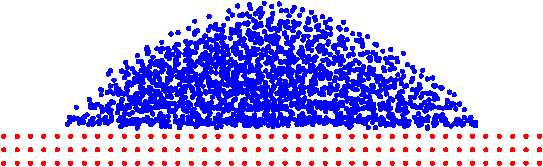
\includegraphics[width=6.7em]{./figures/35.pdf}};
\node[above] at (3.05,-3.5) {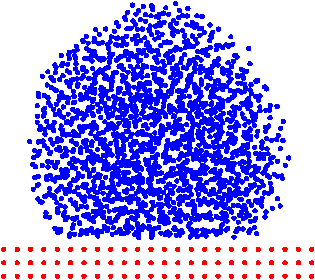
\includegraphics[width=4em]{./figures/20.pdf}};
\end{scope}
\end{tikzpicture}

\end{center}
\end{frame}

\section{细胞的DPD模型和模拟}
\subsection{红细胞的DPD模型和模拟}
\begin{frame}
\frametitle{红细胞膜结构}
\note{\textcolor{red}{330-350s}}
\note[item]{另一方面, 我们还对红细胞的运动与变形进行了模拟}
\note[item]{图8是血红细胞的模结构, 红细胞膜主要由双分子层, 跨膜蛋白及膜下的血影蛋白网组成. 血影蛋白网是细胞的主要骨架}
\begin{figure}[!htb]
\centering
\begin{tikzpicture}[scale=0.7]
\foreach \xf/\yf/\xs/\ys in {
2.9900/5.0400/2.9900/5.0400,
 2.9900/5.0400/4.7900/5.1000,
 2.9900/5.0400/1.3800/3.3900,
 2.9900/5.0400/3.6300/3.7100,
 4.7900/5.1000/4.7900/5.1000,
 4.7900/5.1000/6.9100/5.1300,
 4.7900/5.1000/3.6300/3.7100,
 4.7900/5.1000/5.7100/3.7300,
 6.9100/5.1300/6.9100/5.1300,
 6.9100/5.1300/8.6400/5.0900,
 6.9100/5.1300/5.7100/3.7300,
 6.9100/5.1300/7.9100/3.8600,
 8.6400/5.0900/8.6400/5.0900,
 8.6400/5.0900/10.8100/5.3100,
 8.6400/5.0900/7.9100/3.8600,
 8.6400/5.0900/9.5200/3.8800,
10.8100/5.3100/10.8100/5.3100,
10.8100/5.3100/9.5200/3.8800,
10.8100/5.3100/11.8700/3.7700,
 1.3800/3.3900/1.3800/3.3900,
 1.3800/3.3900/3.6300/3.7100,
 1.3800/3.3900/2.8900/2.1000,
 3.6300/3.7100/3.6300/3.7100,
 3.6300/3.7100/5.7100/3.7300,
 3.6300/3.7100/2.8900/2.1000,
 3.6300/3.7100/4.8100/2.0100,
 5.7100/3.7300/5.7100/3.7300,
 5.7100/3.7300/7.9100/3.8600,
 5.7100/3.7300/4.8100/2.0100,
 5.7100/3.7300/6.9600/2.4900,
 7.9100/3.8600/7.9100/3.8600,
 7.9100/3.8600/9.5200/3.8800,
 7.9100/3.8600/6.9600/2.4900,
 7.9100/3.8600/8.6800/2.2300,
 9.5200/3.8800/9.5200/3.8800,
 9.5200/3.8800/11.8700/3.7700,
 9.5200/3.8800/8.6800/2.2300,
 9.5200/3.8800/10.9100/2.4600,
11.8700/3.7700/11.8700/3.7700,
11.8700/3.7700/10.9100/2.4600,
11.8700/3.7700/12.9800/2.1000,
 0.5400/2.3900/0.5400/2.3900,
 1.3800/3.3900/1.6400/0.5100,
 2.8900/2.1000/2.8900/2.1000,
 2.8900/2.1000/4.8100/2.0100,
 2.8900/2.1000/1.6400/0.5100,
 2.8900/2.1000/3.8300/0.4100,
 4.8100/2.0100/4.8100/2.0100,
 4.8100/2.0100/6.9600/2.4900,
 4.8100/2.0100/3.8300/0.4100,
 4.8100/2.0100/5.6700/0.5300,
 6.9600/2.4900/6.9600/2.4900,
 6.9600/2.4900/8.6800/2.2300,
 6.9600/2.4900/5.6700/0.5300,
 6.9600/2.4900/7.8100/0.9900,
 8.6800/2.2300/8.6800/2.2300,
 8.6800/2.2300/10.9100/2.4600,
 8.6800/2.2300/7.8100/0.9900,
 8.6800/2.2300/9.6900/0.6600,
10.9100/2.4600/10.9100/2.4600,
10.9100/2.4600/12.9800/2.1000,
10.9100/2.4600/9.6900/0.6600,
10.9100/2.4600/11.9900/0.6100,
12.9800/2.1000/12.9800/2.1000,
12.9800/2.1000/11.9900/0.6100,
 1.6400/0.5100/1.6400/0.5100,
 1.6400/0.5100/3.8300/0.4100,
 3.8300/0.4100/3.8300/0.4100,
 3.8300/0.4100/5.6700/0.5300,
 5.6700/0.5300/5.6700/0.5300,
 5.6700/0.5300/7.8100/0.9900,
 7.8100/0.9900/7.8100/0.9900,
 7.8100/0.9900/9.6900/0.6600,
 9.6900/0.6600/9.6900/0.6600,
 9.6900/0.6600/11.9900/0.6100,
11.9900/0.6100/11.9900/0.6100
} {\draw[gray,line width = 5pt,xshift=-51,yshift=-65] (\xf,\yf/2) -- (\xs,\ys/2);}



\foreach \y in {0,0.25,0.5,0.75,1}{
      \ifthenelse{\lengthtest{\y pt = 0.5pt}}{
        \shadedraw [ball color= gray!80] (8.75,0.3) ellipse (0.28 and 0.56);
      }{}
      \ifthenelse{\lengthtest{\y pt = 0.75pt}}{
        \shadedraw [ball color= gray!80] (6,0.0) ellipse (0.28 and 0.56);
      }{}
      \ifthenelse{\lengthtest{\y pt = 0.75pt}}{
        \shadedraw [ball color= gray!80] (1.25,1.2) ellipse (0.28 and 0.56);
      }{}
      \ifthenelse{\lengthtest{\y pt = 1 pt}}{
        \shadedraw [ball color= gray!80] (4,0.9) ellipse (0.28 and 0.56);
      }{}

    \foreach \x  in {1.5,2,2.5,3,3.5,4,4.5,5,5.5,6,6.5,7,7.5,8,8.5,9}{
        \draw[line cap=round, black, line width=1.75pt] (\x-\y+0.15,-\y+0.2) -- (\x-\y+0.15,-\y+1) 
        (\x-\y+0.25,-\y+0.2) .. controls (\x-\y+0.25, -\y+0.6) and (\x-\y+0.25, -\y+0.75) .. (\x-\y+0.3,-\y+1);
        \draw[line cap=round, gray!20, thick] (\x-\y+0.15,-\y+0.2) -- (\x-\y+0.15,-\y+1) 
        (\x-\y+0.25,-\y+0.2) .. controls (\x-\y+0.25, -\y+0.6) and (\x-\y+0.25, -\y+0.75) .. (\x-\y+0.3,-\y+1);
        \shadedraw [ball color= gray!20] (\x-\y,-\y,-0.5) circle (0.25);}


    \foreach \x  in {1.5,2,2.5,3,3.5,4,4.5,5,5.5,6,6.5,7,7.5,8,8.5,9}{
        \draw[line cap=round, black, line width=1.75pt] (\x-\y+0.25,2-\y+0.2) -- (\x-\y+0.25,2-\y-0.7)
        (\x-\y+0.15,2-\y+0.2) .. controls (\x-\y+0.15, 2-\y-0.4) and (\x-\y+0.15, 2-\y-0.45) ..  (\x-\y+0.1,2-\y-0.7);
        \draw[line cap=round, gray!20, thick] (\x-\y+0.25,2-\y+0.2) -- (\x-\y+0.25,2-\y-0.7)
        (\x-\y+0.15,2-\y+0.2) .. controls (\x-\y+0.15, 2-\y-0.4) and (\x-\y+0.15, 2-\y-0.45) ..  (\x-\y+0.1,2-\y-0.7);
        \shadedraw [ball color= gray!20] (\x-\y,2-\y,-0.5) circle (0.25);};
}

     \draw[ball color= gray!60,xshift=27] (2.3031,1.05) arc(-30:210:0.35).. controls (1.9,0.75) and (1.9,0.5) .. (1.9,0.25)
                         -- (1.9,-0.25) .. controls (1.9,-0.5) and (1.9,-0.75)   .. (1.8268,-1) arc(150:390:0.2)
                         .. controls (2.1,-0.75) and (2.1,-0.5) .. (2.1,-0.25) -- (2.1,0.25)
                         .. controls (2.1,0.5) and (2.1,0.75) .. (2.3031,1.05); 
     \draw[ball color= gray!60,yshift=8,xshift=141] (2.1732,1.05) arc(-30:210:0.2).. controls (1.9,0.75) and (1.9,0.5) .. (1.9,0.25)
                         -- (1.9,-0.25) .. controls (1.9,-0.5) and (1.9,-0.75)   .. (1.6969,-1) arc(150:390:0.35)
                         .. controls (2.1,-0.75) and (2.1,-0.5) .. (2.1,-0.25) -- (2.1,0.25)
                         .. controls (2.1,0.5) and (2.1,0.75) .. (2.1732,1.05); 


    \draw[->, >=stealth',very thick](11,2.05)node[right]
        {磷脂双分子层} to[out=195,in=15] (9.5,0.3); 
    \draw[->, >=stealth',very thick](11,2.1)node[right]
        {} to[out=180,in=0] (9.5,2.1); 

     \draw[->, >=stealth',very thick] (11,0.1)node[right]
        {胆固醇} to[out=180,in=0] (9.1,0.1);

     \draw[->, >=stealth',very thick] (11,-1.7)node[right]
        {跨膜蛋白} to[out=180,in=0] (7,-1);
     \draw[->, >=stealth',very thick] (11,-1.75)node[right]
        {} to[out=180,in=-5] (3,-1);

     \draw[->, >=stealth',very thick] (11,-0.8)node[right]
        {血影蛋白网} to[out=180,in=10] (10,-1.1);


\end{tikzpicture}

\caption{\label{fig:RBCstructure} 人类红细胞膜结构}
\end{figure}
\end{frame}

\begin{frame}
\frametitle{网络模型和连续模型}
\note{\textcolor{red}{350-375s}}
\note[item]{我们用左图中由珠簧链构网状结构来模拟红细胞.}
\note[item]{由于目前的实验测出的参数都是基于细胞的连续模型, 如剪切模量, 弯曲刚度. 这些参数需要同粒子模型中的弹簧常数, 弯曲常数等相匹配.}
\begin{figure}[!htb]
\centering
\begin{tikzpicture}
\node at (0,0) {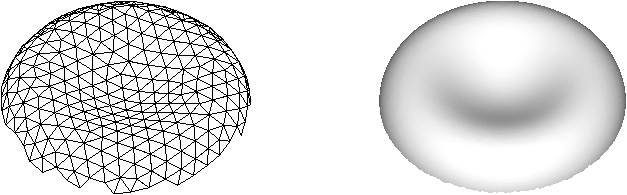
\includegraphics[width=25em]{network2continuum.pdf}};
\node[text width=10em] at (-3,2.2) {\bf 弹簧常数, 弯曲常数, 体积约束, 面积约束};
\node[text width=10em] at ( 3,2.2) {\bf 剪切模量, 压缩模量, 杨氏模量, 弯曲刚度};
\node[text width=5em] at (-2.8,-2) {\bf 粒子模型};
\node[text width=5em] at ( 2.8,-2) {\bf 连续模型};
\draw[very thick, <->, >=stealth'] (-1,2.2) -- (1, 2.2);
\draw[very thick, <->, >=stealth'] (-0.8,0) -- (0.8, 0);
\draw[very thick, <->, >=stealth'] (-1.2,-2) -- (1.2, -2);
\end{tikzpicture}

\caption{\label{fig:network2continuum} 粒子模型(节点为粒子)和连续模型的示意图}
\end{figure}
\end{frame}

\frame{\frametitle{网络模型}
笛卡尔坐标系下的节点$\{\mathbf{x}_i\}, i\in 1\cdots N_v$构成二维三角形网络. 节点间由$N_s$个弹簧构成了$N_t$个三角形. 系统的势能
\[
V(\{\mathbf{X}_i\}) = V_{\text{in-plane}} + V_{\text{bending}} + V_{\text{area}} + V_{\text{volume}}
\]

每个节点的受力
\[
\mathbf{f}_i = -\frac{\partial V(\{\mathbf{x}_i\}) }{\partial \mathbf{x}_i}, \; i\in 1\cdots N_v
\]
}


\frame{\frametitle{面能$V_{\text{in-plane}}$}
膜上弹性能
\[
V_{\text{in-plane}}=\sum_{j\in1\cdots N_s}U_s(l_j)+\sum_{k\in1\cdots N_t} \frac{C_q}{A_k^q}
\]
其中$U_s$可以是$U_{WLC}$, $U_{FENE}$, $\cdots$
\[
U_{WLC}=\frac{K_BTl_m}{4p}\frac{3x^2-2x^3}{1-x}, \; U_{FENE}=-\frac{k_s}{2}l_m^2\log[1-x^2]
\]
其中$x=l/l_m\in(0,1)$, 由平衡时的势能最小可推得
\[
C_q^{WLC}=\frac{\sqrt{3}A_0^{q+1}k_BT(4x_0^2-9x_0+6)}{4pql_m(1-x_0)^2}, \;
C_q^{FENE}=\frac{\sqrt{3}A_0^{q+1}k_s}{q(1-x_0^2)}
\]
}



\frame{\frametitle{弯曲能$V_{\text{bending}}$, 面积能$V_{\text{area}}$和体积能$V_{\text{volume}}$}

\[
V_{\text{bending}}=\sum_{j\in1\cdots N_s}k_b[1-\cos(\theta_j-\theta_0)]
\]

\[
V_{\text{area}}=\frac{k_a(A-A_0^{tot})^2}{2A_0^{tot}} + \sum_{j\in1\cdots N_t}\frac{k_d(A_j-A_0)^2}{2A_0}
\]

\[
V_{\text{volume}}=\frac{k_v(V-V_0^{tot})}{2V_0^{tot}}
\]
}


\begin{frame}
\frametitle{参数匹配: 剪切模量与弹簧常数}
\note{\textcolor{red}{375-390s}}
\note[item]{为了匹配这些参数, 要对珠簧链构成的网络单元进行力学分析, 通过对图10的六边形单元应力分析, 可以得到剪切模量与弹簧常数的关系}
\begin{columns}
\begin{column}[c]{0.5\textwidth}
\begin{figure}[!htb]
\centering
\begin{tikzpicture}[
    scale = 0.7,
    axis/.style={very thick, ->, >=stealth'},
    important line/.style={thick},
    dashed line/.style={dashed},
    pile/.style={thick, ->, >=stealth', shorten <=2pt, shorten
    >=2pt},
    every node/.style={color=black}]
    % axis
    \filldraw[fill=gray!10,draw=gray!10] (15:3) -- 
         (75:3) -- (135:3) -- (195:3) -- (255:3) -- (315:3) -- (375:3);
    \filldraw[fill=gray!30,draw=gray!30] (45:1.732)  -- (105:1.732) -- (165:1.732) -- (225:1.732) -- (285:1.732) -- (345:1.732) -- (405:1.732);
    \draw[axis] (0,0)  -- (4.1,0) node(xline)[right]{$x$};
    \draw[axis] (0,0)  -- (0,3.8) node(yline)[above]{$y$};
    \draw[thick] ( 15:-3) --node[very near end, below]{$a$} ( 15:3) node[right]{$(a_x, a_y)$};
    \draw[thick] ( 75:-3) --node[very near end, right]{$b$} ( 75:3) node[right]{$(b_x, b_y)$};
    \draw[thick] (135:-3) -- (135:3) node[above]{$(c_x, c_y)$};
    \draw[thick] (15:3) -- node[right] {\,$c=|\vec{b}-\vec{a}|$}
         (75:3) -- (135:3) -- (195:3) -- (255:3) -- (315:3) -- (375:3);
    \draw[thick] (45:2.2) node{$\mathbf{A}$} (105:1) node{$\mathbf{S}$} (170:0.4) node{$v$};
    \fill (0,0) circle (2.5pt);
    \draw[densely dashed,thick] (45:1.732)  -- (105:1.732) -- (165:1.732) -- (225:1.732) -- (285:1.732) -- (345:1.732) -- (405:1.732);
\end{tikzpicture}


\caption{\label{fig:network2continuum} 六边形单元}
\end{figure}
\end{column}
\begin{column}[c]{0.5\textwidth}
\begin{figure}[!htb]
\centering
\begin{tikzpicture}[scale = 0.7,rotate around = {15:(0,0,0)},
    axis/.style={very thick, ->, >=stealth'},
    important line/.style={thick},
    dashed line/.style={dashed, thin},
    pile/.style={thick, ->, >=stealth', shorten <=2pt, shorten
    >=2pt},
    every node/.style={color=black}]
    \coordinate (O) at (0,0);
    \coordinate (A) at (4.12,4.64);
    \coordinate (B) at (4.84,1.8);
    \coordinate (C) at (6.48,4.08);
    \coordinate (D) at (7.6,2.0);
    \coordinate (e) at (33.89:6.31);
    \coordinate (f) at (22.67:6.85);
    \coordinate (X) at ($ (B)!.625!(C) $);

    \filldraw[fill=gray!20,draw=gray!20,opacity=0.2] (O) -- (A) -- (C) -- cycle;
    \filldraw[ball color= gray!20,draw=gray!80,opacity=0.2] (O) -- (D) -- (C) -- cycle;
    \filldraw[fill=gray,draw=gray,opacity=0.2] (O) -- (B) -- (C) -- cycle;
    \draw [thick, gray] (O) -- (C) (O)-- node[near end,below]{$S$}(X); 

    \draw [very thick, dashed, black!80] (O) -- (e) (O) -- (f);
    \filldraw[fill=gray!10,draw=gray!10,opacity=0.5] (A) -- (C) -- (B) -- cycle;
    \filldraw[ball color= gray!20,draw=gray!80,opacity=0.5] (D) -- (C) -- (B) -- cycle;

    \draw[thick] (A) -- node[above] {a} (C) -- (B) -- cycle;
    
    \draw[thick] (C)-- (D) -- (B); 
    \draw[thick] (O) -- node[above]{$R$} (A) 
          (O) -- (B) 
          (O) -- node[below]{$R$} (D);
\draw[thick] (e) -- node[near start,below] {$r$} (X) (f) --  node[near start, above] {$r$} (X);
    \draw[black!80] ($ (X)!.15!(C) $) -- ($ (X)!.15!(C)!0.08!-80:(B) $) -- ($ (X)!.2!(e) $)
($ (X)!-.15!(C) $) -- ($ (X)!-.15!(C)!0.08!80:(B) $) -- ($ (X)!.19!(f) $);
    \draw [axis] (e) -- (33.89:9) node[left] {$\mathbf{n}_1$};
    \draw [axis] (f) -- (22.67:8.8) node[above] {$\mathbf{n}_2$};
    \draw (22.67:8.2)  arc(22.67:33.89:8.2) (28:8.5) node{$\theta$};
    \fill (O)    node[left]{$O$}    circle (2.5pt) 
          (33.89:6.31) circle (2pt) 
          (22.67:6.85) circle (2pt);
    \filldraw[fill=gray!20,draw=black,opacity=0.5] (O) -- (A) -- (B) -- cycle;
    \filldraw[ball color= gray!20,draw=black,opacity=0.2] (O) -- (D) -- (B) -- cycle;
\end{tikzpicture}

\vspace{-2em}
\caption{\label{fig:network2continuum} 三角形单元}
\end{figure}
\end{column}
\end{columns}
\end{frame}


\begin{frame}{细胞膜粘性}
细胞膜具有粘弹性, 传统的DPD方法不足以模拟细胞膜的粘性. 在珠簧链模型中加入$-\gamma \mathbf{v}_{ij}$项, 其表达式为
\[
\mathbf{F}_{ij}^D = 
-\bigg(
\gamma^T\mathbf{I} + \gamma^C \mathbf{e}_{ij}\mathbf{e}_{ij}
\bigg)\mathbf{v}_{ij}
=-\gamma^T\mathbf{v}_{ij} -\gamma^C(\mathbf{v}_{ij}\cdot \mathbf{e}_{ij}) \mathbf{e}_{ij}
\]
为了维持系统温度的恒定, 需要增加相应的随机力项
\[
\mathbf{F}^R_{ij} dt = \sqrt{2k_BT}
\bigg(
\sqrt{2 \gamma^T} d\overline{\mathbf{W}_{ij}^S} + \sqrt{3\gamma^C-\gamma^T}\frac{\mathrm{tr}[d\mathbf{W}_{ij}]}{3}\mathbf{I}\bigg)\mathbf{e}_{ij}
\]
其中, $d\mathbf{W}_{ij}^S$为具有独立维纳增量的对称矩阵,  $d\overline{\mathbf{W}_{ij}^S}$为相应的无迹对称矩阵. 膜的剪切粘度$\eta_m$为
\[
\eta_m=\frac{\tau_{xy}}{\dot{\gamma}} = \sqrt{3}\gamma^T+ \sqrt{3}\gamma^C/4
\]
\end{frame}

\begin{frame}
\frametitle{红细胞的运动与变形模拟: 剪切流与泊肃叶流(2D)}
\begin{columns}
\begin{column}[c]{0.5\textwidth}
\begin{figure}
\centering
\begin{overpic}[width=\textwidth]{./animate/shear2d/wall.pdf}
\put(0,0){\animategraphics[width=\textwidth, poster=first,controls,buttonsize=0.8em]{3}{./animate/shear2d/}{0}{21}}
\end{overpic}
\caption{剪切流中的红细胞}
\end{figure}
\end{column}
\begin{column}[c]{0.5\textwidth}
\begin{figure}
\centering
\begin{overpic}[width=\textwidth]{./animate/poise2d/wall.pdf}
\put(0,0){\animategraphics[width=\textwidth, poster=first,controls,buttonsize=0.8em]{3}{./animate/poise2d/}{0}{21}}
\end{overpic}
\caption{泊肃叶流中的红细胞}
\end{figure}
\end{column}
\end{columns}
\end{frame}

\begin{frame}{细胞膜粘附模型}
\begin{center}
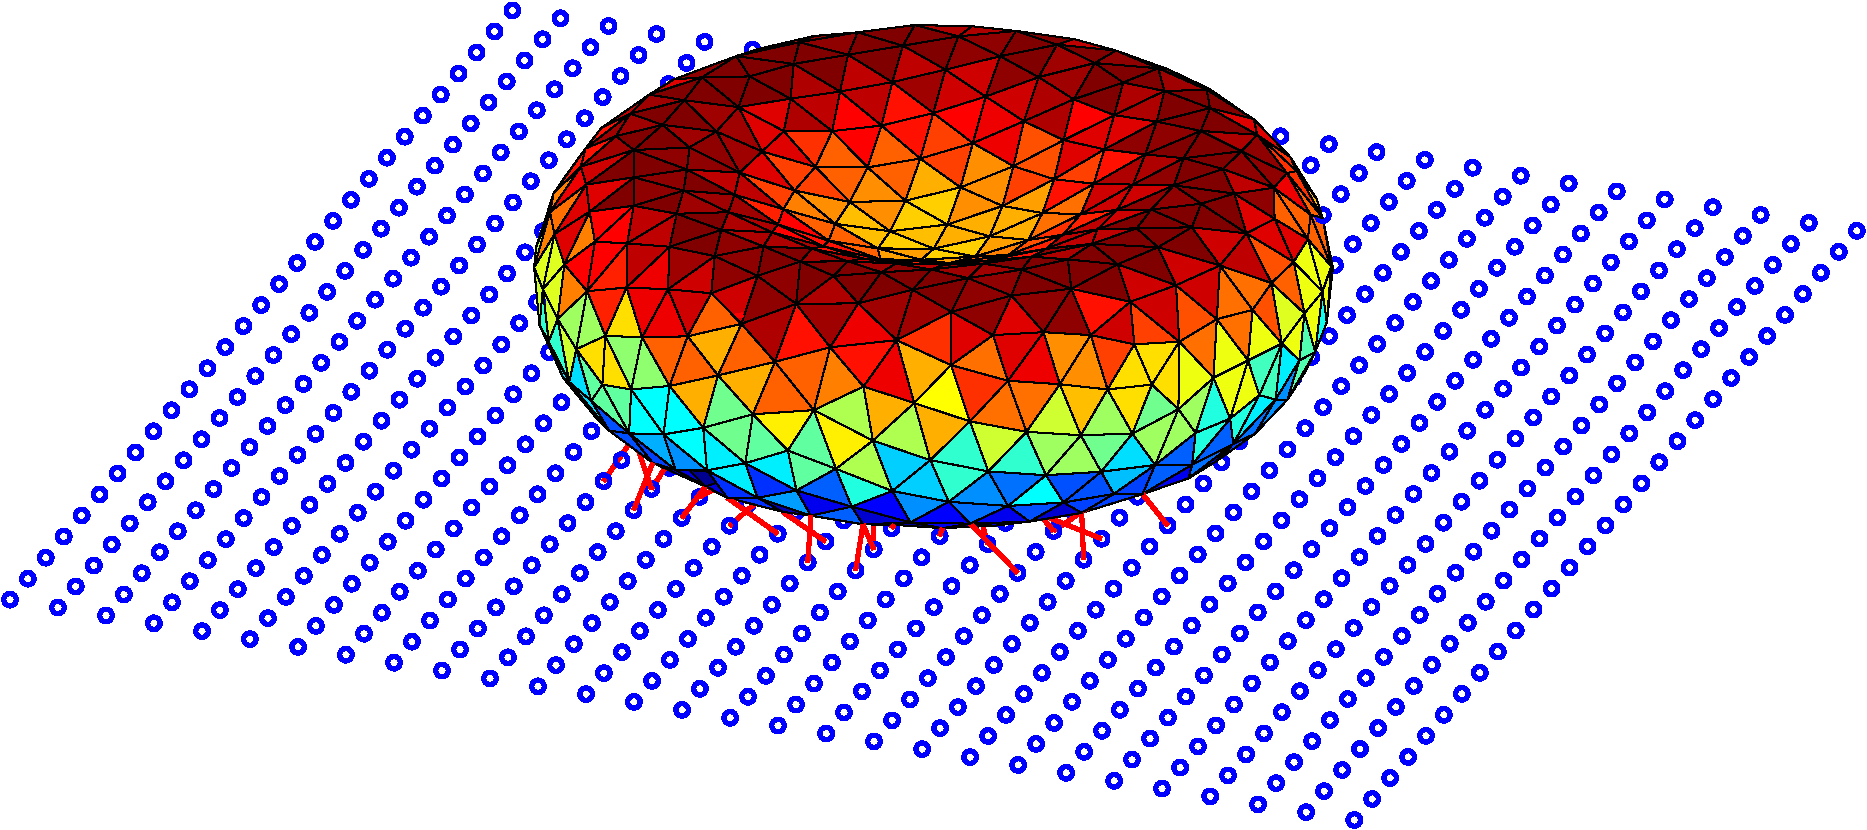
\includegraphics[width=\textwidth]{adhesion.pdf}
\end{center}
\end{frame}

\begin{frame}{细胞膜粘附模型}
配体(细胞膜上的粒子)和受体(壁面上的粒子)间形成bond
\[
F(l) = k_s(l-l_0)
\]
形成bond和断裂bond的概率分别为
\[
P_{on}=\begin{cases}
1-\mathrm{e}^{-k_{\mathrm{on}}\Delta t} & l<d_{\mathrm{on}}\\
0 & l\geq d_{\mathrm{on}}
\end{cases},\quad P_{\mathrm{off}}=\begin{cases}
1-\mathrm{e}^{-k_{\mathrm{off}}\Delta t} & l<d_{off}\\
1 & l\geq d_{\mathrm{off}}
\end{cases}
\]
其中
\[
k_{\mathrm{on}} = k_{\mathrm{on}}^0\exp\bigg(-\frac{\sigma_{\mathrm{on}}(l-l_0)^2}{2k_BT}\bigg),\quad
k_{\mathrm{off}} = k_{\mathrm{off}}^0\exp\bigg(-\frac{\sigma_{\mathrm{off}}(l-l_0)^2}{2k_BT}\bigg)
\]

\end{frame}


\begin{frame}{三维红细胞的拉伸}
\begin{columns}
\begin{column}[c]{0.5\textwidth}
\begin{center}
%\pgfplotsset{compat=1.6}
\newcommand{\rbc}[2]{
\begin{tikzpicture}
\begin{axis}[xmin=-8.5,xmax=8.5,ymin=-4.5,ymax=4.5,width=\textwidth,height=0.8\textwidth,
xticklabel style={font=\scriptsize},
yticklabel style={font=\scriptsize},
xlabel style={font=\footnotesize},
ylabel style={font=\footnotesize},
xlabel={force = #2 pN},
colormap={bw}{gray(0cm)=(0); gray(1cm)=(1)}, view={0}{90},axis equal]
\addplot3[patch] file{./animate/stretch/data/#1};
\end{axis}

\begin{axis}[yshift=-0.55\textwidth,xmin=-8.5,xmax=8.5,zmin=-3,zmax=3,width=\textwidth,height=0.6\textwidth,
zticklabel style={font=\scriptsize},
xticklabel style={font=\scriptsize},
xlabel style={font=\footnotesize},
zlabel style={font=\footnotesize},
colormap={bw}{gray(0cm)=(0); gray(1cm)=(1)}, view={0}{0}, axis equal]
\addplot3[patch] file{./animate/stretch/data/#1};
\end{axis}
\end{tikzpicture}
}

\begin{animateinline}[autoplay,poster=last,controls,buttonsize=0.8em]{3}
%\rbc{2-1txt}{0}\newframe
%\rbc{2-11txt}{20}\newframe
%\rbc{4-11txt}{40}\newframe
%\rbc{6-11txt}{60}\newframe
%\rbc{8-11txt}{80}\newframe
%\rbc{10-11txt}{100}\newframe
%\rbc{12-11txt}{120}\newframe
%\rbc{14-11txt}{140}\newframe
%\rbc{16-11txt}{160}\newframe
%\rbc{18-11txt}{180}\newframe
\rbc{20-11txt}{200}
\end{animateinline}

\animategraphics[width=\textwidth,poster=first,controls,buttonsize=0.8em,autoplay,loop]{2}{./animate/stretch/}{0}{10}
\end{center}

\end{column}
\begin{column}[c]{0.5\textwidth}
\begin{tikzpicture}[scale=0.925]
\begin{axis}[xmin=0,xmax=200,ymin=0,ymax=22,width=182pt,height=1.44\textwidth,xlabel={force ($\mathrm{pN}$)},ylabel={diameter ($\mathrm{\mu m}$)},
ytick={0,2,...,20},
label style={anchor=near ticklabel},
    ylabel style={yshift=-2em},
    xlabel style={yshift=0.3em},
    tick label style={font=\scriptsize },
    label style={font=\footnotesize},
    legend style={font=\tiny,legend cell align=left,legend pos=north west}
]


\addplot+[mark=diamond,only marks,error bars/.cd,
	y dir=both,y explicit]
coordinates {
(  0.01,  7.820) +- (0,0.780)
( 16.41,  9.230) +- (0,0.880)
( 19.70,  9.535) +- (0,0.935)
( 31.01, 10.455) +- (0,0.955)
( 38.30, 11.145) +- (0,1.145)
( 47.11, 11.870) +- (0,1.090)
( 67.51, 12.860) +- (0,1.070)
( 87.60, 13.775) +- (0,1.225)
(108.99, 14.390) +- (0,1.470)
(130.01, 15.190) +- (0,1.450)
(151.01, 15.610) +- (0,1.300)
(173.00, 16.065) +- (0,1.815)
(192.99, 16.255) +- (0,1.795)
(  0.01,  7.515) +- (0,0.705)
( 16.41,  6.195) +- (0,0.665)
( 19.70,  6.260) +- (0,0.710)
( 31.01,  5.760) +- (0,0.570)
( 38.30,  5.405) +- (0,0.595)
( 47.11,  5.090) +- (0,0.820)
( 67.51,  4.695) +- (0,0.735)
( 87.60,  4.665) +- (0,0.635)
(108.99,  4.595) +- (0,0.715)
(130.01,  4.575) +- (0,0.635)
(151.01,  4.405) +- (0,0.605)
(173.00,  4.580) +- (0,0.510)
(192.99,  4.395) +- (0,0.615)};

\addlegendentry{Experiment}

\addplot+[no marks,red,smooth] table[x=x,y=y]{./figures/data/spectrin.dat};
\addlegendentry{spectrin-level, Dao et al.}

\addplot+[no marks,black,densely dashed,smooth,thick] table[x=f,y=w]{./figures/data/wlc-pow.dat};
\addlegendentry{wlc-pow, $N_v = 500$}

\addplot+[no marks,black,densely dotted,smooth,thick] table[x=f,y=w]{./figures/data/fene-pow.dat};
\addlegendentry{fene-pow, $N_v = 500$}

\node[font=\footnotesize] at (axis cs:170,7){$D_T$};
\node[font=\footnotesize] at (axis cs:170,12.5){$D_A$};

\end{axis}
\end{tikzpicture}

\vspace{-2.6em}
\end{column}
\end{columns}
\end{frame}

\begin{frame}{剪切流中的三维红细胞, $\dot{\gamma}=10 \mathrm{s}^{-1}$}
\begin{columns}
\begin{column}[c]{0.5\textwidth}
\begin{center}
\animategraphics[width=\textwidth,poster=first,controls,buttonsize=0.8em,autoplay,loop]{5}{./animate/shear10/}{1}{71}
\end{center}
\end{column}
\begin{column}[c]{0.5\textwidth}
\begin{tikzpicture}[scale=0.925]
\begin{axis}[xmin=0,xmax=200,ymin=0,ymax=50,width=182pt,height=1.44\textwidth,
xlabel={$\dot{\gamma}$ ($\mathrm{s}^{-1}$)},ylabel={Frequency ($\mathrm{rad/s}$)},
label style={anchor=near ticklabel},
    ylabel style={yshift=-2em},
    xlabel style={yshift=0.3em},
    tick label style={font=\scriptsize },
    label style={font=\footnotesize},
legend style={font=\tiny,legend cell align=left,legend pos=north west}
]

\fill[blue!50,opacity=0.25] (axis cs:0,0)--(axis cs:30,0)--(axis cs:30,50)--(axis cs:0,50)--cycle;
\fill[red!50,opacity=0.25] (axis cs:30,0)--(axis cs:50,0)--(axis cs:50,50)--(axis cs:30,50)--cycle;
\fill[green!50,opacity=0.25] (axis cs:50,0)--(axis cs:200,0)--(axis cs:200,50)--(axis cs:50,50)--cycle;
\addplot+[mark=diamond,error bars/.cd,
	y dir=both,y explicit]
coordinates {
(28.6, 6.22) +- (0,0.31)
(42.9, 9.42) +- (0,0.57)
(57.1,12.70) +- (0,0.57)
(114.3,24.6) +- (0,1.07)
(171.4,37.4) +- (0,1.45)};

\addlegendentry{Tran-Son-Tay et al. (1984)};

\addplot+[no marks,thick,black] table[x=x,y=y]
{x    y
 0    0
 10   2   
 20   4.5
 30   7
 40   8
 50   9
 60   11.3
 70   13.6
 80   15.8
 90   18.1
100   20.4
110   22.7
120   25
130   27.3
140   29.6
150   31.9
160   34.1
170   36.4
180   38.7
190   41
};
\addlegendentry{wlc-pow, $N_v=500$}


\node[font=\scriptsize,left] at (axis cs:190,3){$\eta_{\textrm{i}} = \eta_{\textrm{o}} = 5.0\times 10^{-3}~ \mathrm{Pa\cdot s}$};
\node[font=\scriptsize,left] at (axis cs:190,7){$\eta_{\textrm{m}} = 2.2\times 10^{-2}~\mathrm{Pa\cdot s}$};


\node[font=\scriptsize,right,rotate=90,blue] at (axis cs:15,25){Tumbling};
\node[font=\scriptsize,right,rotate=90,red] at (axis cs:40,25){Intermittent};
\node[font=\scriptsize,right,rotate=90,green!40!black] at (axis cs:100,25){Tank-Treading};
\end{axis}
\end{tikzpicture}

\vspace{-2.6em}
\end{column}
\end{columns}
\end{frame}

\begin{frame}{剪切流中的三维红细胞, $\dot{\gamma}=30 \mathrm{s}^{-1}$}
\begin{columns}
\begin{column}[c]{0.5\textwidth}
\begin{center}
\animategraphics[width=\textwidth,poster=first,controls,buttonsize=0.8em,autoplay,loop]{5}{./animate/shear30/}{1}{59}
\end{center}
\end{column}
\begin{column}[c]{0.5\textwidth}
\begin{tikzpicture}[scale=0.925]
\begin{axis}[xmin=0,xmax=200,ymin=0,ymax=50,width=182pt,height=1.44\textwidth,
xlabel={$\dot{\gamma}$ ($\mathrm{s}^{-1}$)},ylabel={Frequency ($\mathrm{rad/s}$)},
label style={anchor=near ticklabel},
    ylabel style={yshift=-2em},
    xlabel style={yshift=0.3em},
    tick label style={font=\scriptsize },
    label style={font=\footnotesize},
legend style={font=\tiny,legend cell align=left,legend pos=north west}
]

\fill[blue!50,opacity=0.25] (axis cs:0,0)--(axis cs:30,0)--(axis cs:30,50)--(axis cs:0,50)--cycle;
\fill[red!50,opacity=0.25] (axis cs:30,0)--(axis cs:50,0)--(axis cs:50,50)--(axis cs:30,50)--cycle;
\fill[green!50,opacity=0.25] (axis cs:50,0)--(axis cs:200,0)--(axis cs:200,50)--(axis cs:50,50)--cycle;
\addplot+[mark=diamond,error bars/.cd,
	y dir=both,y explicit]
coordinates {
(28.6, 6.22) +- (0,0.31)
(42.9, 9.42) +- (0,0.57)
(57.1,12.70) +- (0,0.57)
(114.3,24.6) +- (0,1.07)
(171.4,37.4) +- (0,1.45)};

\addlegendentry{Tran-Son-Tay et al. (1984)};

\addplot+[no marks,thick,black] table[x=x,y=y]
{x    y
 0    0
 10   2   
 20   4.5
 30   7
 40   8
 50   9
 60   11.3
 70   13.6
 80   15.8
 90   18.1
100   20.4
110   22.7
120   25
130   27.3
140   29.6
150   31.9
160   34.1
170   36.4
180   38.7
190   41
};
\addlegendentry{wlc-pow, $N_v=500$}


\node[font=\scriptsize,left] at (axis cs:190,3){$\eta_{\textrm{i}} = \eta_{\textrm{o}} = 5.0\times 10^{-3}~ \mathrm{Pa\cdot s}$};
\node[font=\scriptsize,left] at (axis cs:190,7){$\eta_{\textrm{m}} = 2.2\times 10^{-2}~\mathrm{Pa\cdot s}$};


\node[font=\scriptsize,right,rotate=90,blue] at (axis cs:15,25){Tumbling};
\node[font=\scriptsize,right,rotate=90,red] at (axis cs:40,25){Intermittent};
\node[font=\scriptsize,right,rotate=90,green!40!black] at (axis cs:100,25){Tank-Treading};
\end{axis}
\end{tikzpicture}

\vspace{-2.6em}
\end{column}
\end{columns}
\end{frame}

\begin{frame}{剪切流中的三维红细胞, $\dot{\gamma}=100 \mathrm{s}^{-1}$}
\begin{columns}
\begin{column}[c]{0.5\textwidth}
\begin{center}
\animategraphics[width=\textwidth,poster=first,controls,buttonsize=0.8em,autoplay,loop]{5}{./animate/shear/}{0}{70}
\end{center}
\end{column}
\begin{column}[c]{0.5\textwidth}
\begin{tikzpicture}[scale=0.925]
\begin{axis}[xmin=0,xmax=200,ymin=0,ymax=50,width=182pt,height=1.44\textwidth,
xlabel={$\dot{\gamma}$ ($\mathrm{s}^{-1}$)},ylabel={Frequency ($\mathrm{rad/s}$)},
label style={anchor=near ticklabel},
    ylabel style={yshift=-2em},
    xlabel style={yshift=0.3em},
    tick label style={font=\scriptsize },
    label style={font=\footnotesize},
legend style={font=\tiny,legend cell align=left,legend pos=north west}
]

\fill[blue!50,opacity=0.25] (axis cs:0,0)--(axis cs:30,0)--(axis cs:30,50)--(axis cs:0,50)--cycle;
\fill[red!50,opacity=0.25] (axis cs:30,0)--(axis cs:50,0)--(axis cs:50,50)--(axis cs:30,50)--cycle;
\fill[green!50,opacity=0.25] (axis cs:50,0)--(axis cs:200,0)--(axis cs:200,50)--(axis cs:50,50)--cycle;
\addplot+[mark=diamond,error bars/.cd,
	y dir=both,y explicit]
coordinates {
(28.6, 6.22) +- (0,0.31)
(42.9, 9.42) +- (0,0.57)
(57.1,12.70) +- (0,0.57)
(114.3,24.6) +- (0,1.07)
(171.4,37.4) +- (0,1.45)};

\addlegendentry{Tran-Son-Tay et al. (1984)};

\addplot+[no marks,thick,black] table[x=x,y=y]
{x    y
 0    0
 10   2   
 20   4.5
 30   7
 40   8
 50   9
 60   11.3
 70   13.6
 80   15.8
 90   18.1
100   20.4
110   22.7
120   25
130   27.3
140   29.6
150   31.9
160   34.1
170   36.4
180   38.7
190   41
};
\addlegendentry{wlc-pow, $N_v=500$}


\node[font=\scriptsize,left] at (axis cs:190,3){$\eta_{\textrm{i}} = \eta_{\textrm{o}} = 5.0\times 10^{-3}~ \mathrm{Pa\cdot s}$};
\node[font=\scriptsize,left] at (axis cs:190,7){$\eta_{\textrm{m}} = 2.2\times 10^{-2}~\mathrm{Pa\cdot s}$};


\node[font=\scriptsize,right,rotate=90,blue] at (axis cs:15,25){Tumbling};
\node[font=\scriptsize,right,rotate=90,red] at (axis cs:40,25){Intermittent};
\node[font=\scriptsize,right,rotate=90,green!40!black] at (axis cs:100,25){Tank-Treading};
\end{axis}
\end{tikzpicture}

\vspace{-2.6em}
\end{column}
\end{columns}
\end{frame}


\begin{frame}{多个红细胞管道流动}
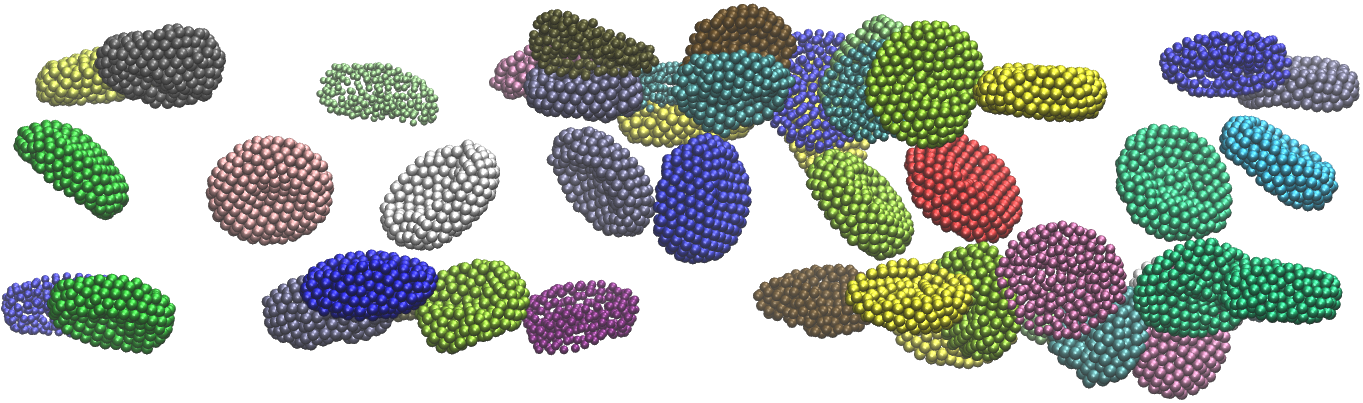
\includegraphics[width=\textwidth]{./figures/rbc.png}
\end{frame}

\subsection{乳腺细胞的模拟}
\begin{frame}{乳腺细胞吸入实验及DPD模型}
\begin{columns}
\begin{column}[c]{0.25\textwidth}
\begin{center}
\usetikzlibrary{%
    decorations.pathreplacing,%
    decorations.pathmorphing,arrows
}
\begin{tikzpicture}
\begin{axis}[axis equal,colormap={bw}{gray(0cm)=(0); gray(1cm)=(1)}, view={0}{90},xmin=-10.25,xmax=10.25,ymin=-10.25,ymax=10.25,width=1.3\textwidth,height=1.3\textwidth,xtick=\empty,ytick=\empty,hide axis]
\addplot3 + [only marks,mark=ball,ball color=gray,draw=none,mark size=1.5pt] table[x=x,y=y,z=z]{./figures/data/sphere.vertex};
\addplot3[patch] file{./figures/data/sphere.dat};
\end{axis}
\end{tikzpicture}

\end{center}
\end{column}
\begin{column}[c]{0.75\textwidth}
{\small
\[
V(\{\mathbf{X}_i\}) = V_{\text{in-plane}} + V_{\text{bending}} + \textcolor{red}{V_{\text{area}}} + V_{\text{volume}}
\]}
\end{column}
\end{columns}
\begin{center}
\asyinclude[width=\textwidth, viewportwidth=\textwidth,viewportheight=0.3571\textwidth]{./figures/3dchannel.asy}
\end{center}
\end{frame}

\begin{frame}{乳腺细胞吸入实验的模拟动画}
\begin{center}
\begin{overpic}[width=\textwidth]{./animate/cell2d/wall.pdf}
\put(0,0){\animategraphics[width=\textwidth, poster=first,controls,buttonsize=0.8em]{5}{./animate/cell2d/}{0}{90}}
\end{overpic}
\end{center}
\end{frame}

\begin{frame}{乳腺细胞吸入实验的模拟结果}
\begin{columns}
\begin{column}[c]{0.5\textwidth}
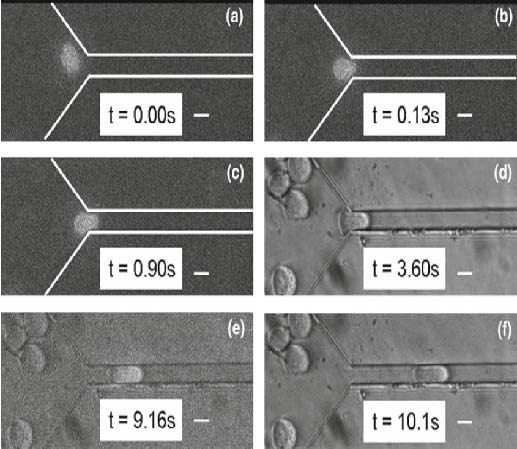
\includegraphics[width=\textwidth]{./figures/cell.jpg}
\end{column}
\begin{column}[c]{0.5\textwidth}
\begin{center}
\usetikzlibrary{%
    decorations.pathreplacing,%
    decorations.pathmorphing,arrows
}
\begin{tikzpicture}[scale=0.925]
\begin{scope}[yshift=95pt]
  \begin{axis}[xmin=-60, xmax=60, ymin=-22, ymax=22,width=182pt,height=95pt,
              ytick={-20,0,20},
              %xlabel={$t$}, 
              ylabel={$z$},
              xticklabel=\empty,
label style={anchor=near ticklabel},
    ylabel style={yshift=-2em},
    xlabel style={yshift=0.3em},
    tick label style={font=\scriptsize},
    label style={font=\footnotesize},
    legend style={font=\tiny,legend cell align=left,legend pos=north west}
              ]

   \addplot[color=black,no marks,thick] coordinates {(-70,-20.25) (-40,-20.25) (-23, -3.25) (23, -3.25) (40,-20.25) (70,-20.25)};
   \addplot[color=black,no marks,thick] coordinates {(-70,20.25) (-40,20.25) (-23, 3.25) (23, 3.25) (40,20.25) (70,20.25)};

   \addplot[no marks,ball color=red]  table[x=x1,y=y1]{./figures/data/cellshape.dat};
   \addplot[no marks, blue!25!red,thick]  table[x=x2,y=y2]{./figures/data/cellshape.dat};
   \addplot[no marks, blue!50!red,thick]  table[x=x3,y=y3]{./figures/data/cellshape.dat};
   \addplot[no marks, blue!75!red,thick]  table[x=x4,y=y4]{./figures/data/cellshape.dat};
   \addplot[no marks, blue!100!red,thick]  table[x=x5,y=y5]{./figures/data/cellshape.dat};
   \addplot[no marks, blue!75!green,thick]  table[x=x6,y=y6]{./figures/data/cellshape.dat};
   \addplot[no marks, blue!50!green,thick]  table[x=x7,y=y7]{./figures/data/cellshape.dat};
   \addplot[no marks, blue!25!green,thick]  table[x=x8,y=y8]{./figures/data/cellshape.dat};
   \addplot[no marks, green,thick]  table[x=x9,y=y9]{./figures/data/cellshape.dat};
   \addplot[no marks, red!25!green,thick]  table[x=x10,y=y10]{./figures/data/cellshape.dat};
   \addplot[no marks, red!50!green,thick]  table[x=x11,y=y11]{./figures/data/cellshape.dat};
   \addplot[no marks, red!75!green,thick]  table[x=x12,y=y12]{./figures/data/cellshape.dat};
  \end{axis}
\end{scope}

  \begin{axis}[xmin=-60, xmax=60, ymin=0, ymax=18, width=182pt,height=135pt,
              %ytick={0,30,60,90,120,150,180},
              xlabel={$x$}, ylabel={$t$},
label style={anchor=near ticklabel},
    ylabel style={yshift=-2em},
    xlabel style={yshift=0.3em},
    tick label style={font=\scriptsize},
    label style={font=\footnotesize},
    legend style={font=\tiny,legend cell align=left,legend pos=north west}
              ]
   \addplot[no marks, black,thick]  table[x=x,y=t]{./figures/data/cellx.dat};

  \end{axis}
\end{tikzpicture}

\vspace{-2em}
\end{center}
\end{column}
\end{columns}
\end{frame}



\section{间质流动中的细胞,基质及间质流体的流固耦合}
\subsection{圆球和圆柱绕流}
\begin{frame}{圆球和圆柱绕流}
\begin{columns}
\begin{column}[c]{0.5\textwidth}
\begin{center}
\begin{tikzpicture}[scale=0.925]
\begin{loglogaxis}[xmin=0.1,xmax=1000,ymin=0.1,ymax=1000,width=180pt,height=180pt,
xlabel=$\mathrm{Re}$,ylabel=$C_d$,
label style={anchor=near ticklabel},
    ylabel style={yshift=-1.5em},
    xlabel style={yshift=0.3em},
    tick label style={font=\scriptsize },
    label style={font=\footnotesize},
    legend style={font=\tiny,legend cell align=left,legend pos=north east},
    title={圆柱绕流阻力系数与雷诺数的关系},
    title style={font=\footnotesize,color=blue}
]

\addplot[only marks, draw=black, fill=black!30, mark size=1.5] coordinates {
(    0.2076,   32.325)
(    1.0185,   7.1251)
(    3.8097,    2.4983)
(    9.9904,    1.5399)
(   17.9616,    1.2368)
(  85.9442,    1.1305)
};
\addlegendentry{DPD}



\addplot+[mark=none,domain=0.1:1000,samples=2,densely dashed,red] {6/x}; 
\addlegendentry{$6/\mathrm{Re}$}

\addplot[mark=none,blue,smooth]  table[x=Re,y=Cd]{./figures/data/cylinderCdExperiment.dat};
\addlegendentry{实验拟合曲线}


\end{loglogaxis}
\end{tikzpicture}

\end{center}
\end{column}
\begin{column}[c]{0.5\textwidth}
\begin{center}
\begin{tikzpicture}[scale=0.925]
\begin{loglogaxis}[xmin=0.1,xmax=1000,ymin=0.01,ymax=10000,width=180pt,height=180pt,
xlabel=$\mathrm{Re}$,ylabel=$C_d$,
label style={anchor=near ticklabel},
    ylabel style={yshift=-1.5em},
    xlabel style={yshift=0.3em},
    tick label style={font=\scriptsize },
    label style={font=\footnotesize},
    legend style={font=\tiny,legend cell align=left,legend pos=north east},
    title={圆球绕流阻力系数与雷诺数的关系},
    title style={font=\footnotesize,color=blue}
]

\addplot[only marks, draw=black, fill=black!30, mark size=1.5] coordinates {
		( 0.20,112.34)
                ( 0.99, 27.33)
                ( 2.10, 13.01)
                ( 4.02,  7.04)
                ( 9.80,  3.28)
                ( 22.00, 2.02)
                ( 40.98, 1.31)
                ( 81.32, 0.98)
                (101.25, 0.99)};


%\addplot[only marks, draw=black, fill=black!30, mark size=1.5] coordinates {
%(4.5044,    7.7161)
%(20.8442,    2.6203)
%(39.1188,    2.1084)
%(69.8477,   2.2380)};
\addlegendentry{DPD}

\addplot+[mark=none,domain=0.1:1000,samples=2,densely dashed,red] {24/x}; 
\addlegendentry{$24/\mathrm{Re}$}
%\addlegendentry{$\frac{24}{\mathrm{Re}}$}

\addplot+[mark=none,domain=0.2:1000,samples=200,smooth,blue] {21.12/x + 6.3/sqrt(x) + 0.25}; 
\addlegendentry{实验拟合曲线}
%\addlegendentry{$21.12/\mathrm{Re}+6.3/\sqrt{\mathrm{Re}}+0.25$}
%\addlegendentry{$\frac{21.12}{\mathrm{Re}}+\frac{6.3}{\sqrt{\mathrm{Re}}}+0.25$}
\end{loglogaxis}
\end{tikzpicture}

\end{center}
\end{column}
\end{columns}
\end{frame}

\subsection{三维纤维阵列构造}
\begin{frame}{平行}
\asyinclude[width=0.6\textwidth, viewportwidth=\textwidth,viewportheight=0.6\textwidth]{./figures/parallel.asy}
\end{frame}
\begin{frame}{垂直}
\asyinclude[width=0.6\textwidth, viewportwidth=\textwidth,viewportheight=0.6\textwidth]{./figures/perpendicular.asy}
\end{frame}
\begin{frame}{立体网格}
\asyinclude[width=0.6\textwidth, viewportwidth=\textwidth,viewportheight=0.6\textwidth]{./figures/cubic.asy}
\end{frame}

\subsection{初步计算结果}
\begin{frame}{圆球和圆柱绕流}
\begin{columns}
\begin{column}[c]{0.5\textwidth}
\begin{center}
\begin{tikzpicture}[scale=0.925]
\begin{axis}[xmin=0.01, xmax=0.05, ymin=100, ymax=600, width=182pt, height=180pt,
xlabel=$g$,ylabel=$F_\mathrm{drag}$,
label style={anchor=near ticklabel},
    ylabel style={yshift=-2em},
    xlabel style={yshift=0.3em},
    tick label style={font=\scriptsize },
    label style={font=\footnotesize},
    legend style={font=\tiny,legend cell align=left,legend pos=north east},
    title={水平体力(压差)与流体阻力},
    title style={font=\footnotesize,color=blue}
]

\addplot[mark=*, mark options={fill=black!30}, mark size=1.5, draw=black] coordinates {
    (0.0100,  218.8612)
    (0.0200,  278.9519)
    (0.0300,  319.1112)
    (0.0400,  363.4497)
    (0.0500,  378.0218)};

\addlegendentry{parallel};


\addplot[mark=*, mark options={fill=blue!30}, mark size=1.5, draw=blue] coordinates {
    (0.0100,  109.5405)
    (0.0200,  139.6161)
    (0.0300,  161.5611)
    (0.0400,  183.7822)
    (0.0500,  194.0888)};
\addlegendentry{perpendicular};


\addplot[mark=*, mark options={fill=red!30}, mark size=1.5, draw=red] coordinates {
    (0.0100,  126.2987)
    (0.0200,  160.9754)
    (0.0300,  183.9844)
    (0.0400,  208.4314)
    (0.0500,  212.3290)
};
\addlegendentry{cubic};

\end{axis}
\end{tikzpicture}

\end{center}
\end{column}
\begin{column}[c]{0.5\textwidth}
\begin{center}
\begin{tikzpicture}[scale=0.925]
\begin{axis}[xmin=0.01, xmax=0.05, ymin=0, ymax=3, width=182pt, height=180pt,
xlabel=$g$,ylabel=$v_\mathrm{mean}$,
label style={anchor=near ticklabel},
    ylabel style={yshift=-2em},
    xlabel style={yshift=0.3em},
    tick label style={font=\scriptsize },
    label style={font=\footnotesize},
    legend style={font=\tiny,legend cell align=left,legend pos=north east},
    title={水平体力(压差)与平均流速},
    title style={font=\footnotesize,color=blue}
]

\addplot[mark=*, mark options={fill=black!30}, mark size=1.5, draw=black] coordinates {
    (0.0100,    0.2858)
    (0.0200,    0.5715)
    (0.0300,    0.8444)
    (0.0400,    1.1563)
    (0.0500,    1.4760)};

\addlegendentry{parallel};


\addplot[mark=*, mark options={fill=blue!30}, mark size=1.5, draw=blue] coordinates {
    (0.0100,    0.0394)
    (0.0200,    0.0789)
    (0.0300,    0.1148)
    (0.0400,    0.1574)
    (0.0500,    0.1989)};
\addlegendentry{perpendicular};


\addplot[mark=*, mark options={fill=red!30}, mark size=1.5, draw=red] coordinates {
    (0.0100,    0.0588)
    (0.0200,    0.1176)
    (0.0300,    0.1720)
    (0.0400,    0.2317)
    (0.0500,    0.2955)
};
\addlegendentry{cubic};


\addplot[mark=*,  mark options={fill=black!30}, mark size=1.5, draw=black] coordinates {
    (0.0100,    1.253)
    (0.0200,    2.447)};

\end{axis}
\end{tikzpicture}

\end{center}
\end{column}
\end{columns}
\end{frame}



%\section<presentation>*{参考文献}

\frame[plain]{
  \transdissolve
  \frametitle<presentation>{参考文献}

  \beamertemplatebookbibitems
  \beamertemplatearticlebibitems
  \begin{thebibliography}{10}
  \bibitem{userguide} Zhou L. V., Liu M. B. and Chang J. Z., Interaction 
  \bibitem{userguide} Liu M.B., Liu G.R., Zhou L. V. and Chang J. Z., Archives of Computational Methods in Engineering, 2014.and Multiscale Mechanics 6(2): 157-172, 2013.
  \bibitem{userguide} Pivkin, I. V., and G. E. Karniadakis. 2008. Accurate coarse-grained modeling of red blood cells. Phys. Rev. Lett. 101:118105.
  \bibitem{TeX} Fedosov, D. A. 2010. Multiscale modeling of blood flow and soft matter. PhD thesis, Brown University, Providence, RI.
  \bibitem{TeX} Tran-Son-Tay, R., S. P. Sutera, and P. R. Rao. 1984. Determination of red blood cell membrane viscosity from rheoscopic observations of tank-treading motion. Biophys. J. 46:65–72.
  %\bibitem{userguide} 周吕文, 刘谋斌, 常建忠. 颗粒材料计算力学研究进展. 2012:625-633.
  \bibitem{TeX} Leong FY,Li Q, Lim CT, Chiam K-H (2011) Modeling cell entry into a micro-channel. Biomechanics and modeling in mechanobiology 10(5):755-766.
  \end{thebibliography}
}

%%%%%%%%%%%%%%%%%%%%%%%%%%%%%%%%%%%%%%%%%%%%%%%%%%%%%%%%%%%%%%%%%%%%%%%%%%
\plainframe{
    \begin{centering}
      \Huge Thank You!!!\par
    \end{centering}
  } 

\end{document}
